% This template was initially provided by Dulip Withanage.
% Modifications for the database systems research group
% were made by Conny Junghans,  Jannik Strötgen and Michael Gertz

\documentclass[
     12pt,         % font size
     a4paper,      % paper format
     BCOR10mm,     % binding correction
     DIV14,        % stripe size for margin calculation
     ]{article}

%%%%%%%%%%%%%%%%%%%%%%%%%%%%%%%%%%%%%%%%%%%%%%%%%%%%%%%%%%%%

% PACKAGES:

% Use German :
\usepackage[english]{babel}
% Input and font encoding
\usepackage[latin1]{inputenc}
\usepackage[T1]{fontenc}
% Index-generation
\usepackage{makeidx}
% Einbinden von URLs:
\usepackage{url}
% Special \LaTex symbols (e.g. \BibTeX):
%\usepackage{doc}
% Include Graphic-files:
\usepackage{graphicx}
% Include doc++ generated tex-files:
%\usepackage{docxx}

% Fuer anderthalbzeiligen Textsatz
\usepackage{setspace}

% Fuer research questions
\usepackage{enumitem}

\newlist{questions}{enumerate}{2}
\setlist[questions,1]{label=RQ\arabic*.,ref=RQ\arabic*}
\setlist[questions,2]{label=(\alph*),ref=\thequestionsi(\alph*)}

% hyperrefs in the documents
 \PassOptionsToPackage{hyphens}{url}\usepackage[bookmarks=true,colorlinks,pdfpagelabels,pdfstartview = FitH,bookmarksopen = true,bookmarksnumbered = true,linkcolor = black,plainpages = false,hypertexnames = false,citecolor = black,urlcolor=black]{hyperref}
 \usepackage{hyperref}
 \def\UrlBreaks{\do\/\do-}
%%%%%%%%%%%%%%%%%%%%%%%%%%%%%%%%%%%%%%%%%%%%%%%%%%%%%%%%%%%%

% OTHER SETTINGS:

% Choose language
\newcommand{\setlang}[1]{\selectlanguage{#1}\nonfrenchspacing}


\begin{document}

% TITLE:
\pagenumbering{roman} 
\begin{titlepage}


\vspace*{1cm}
\begin{center}
\vspace*{3cm}
\textbf{ 
\Large Heidelberg University\\
\smallskip
\Large Institute of Computer Science\\
%\smallskip
%\Large Database Systems Research Group\\
\smallskip
}

\vspace{3cm}

\textbf{\large Project Proposal for the lecture \\  Data Science for Text Analytics}

\vspace{0.5\baselineskip}
{\huge
\textbf{Hate, Discrimination \& Racism in German Rap - A Text Analytics Approach}
}
\end{center}

\vfill 

{\large
\begin{tabular}[l]{ll}
Johannes Sindlinger: & 3729339, Computer and Data Science, M. Sc.\\
  & johannes.sindlinger@stud.uni-heidelberg.de\\
Mara-Eliana Popescu: & 4166979, Computer Science, B. Sc. \\
  & mara-eliana.popescu@stud.uni-heidelberg.de\\
Team Member: & Name, Matriculation Number, Course of Study\\
  & email address\\

% If the line goes too far to the right, you can alter this slightly, e.g.
Team Member: & Very long Name, Matriculation Number\\
  & Course of Study, email address\\
  
\end{tabular}
}

\end{titlepage}

\pagenumbering{arabic} 

\section{Motivation}
'I leave no whore daughter unfucked, everyone wants my dick - even lesbians get turned around!' - Excerpts from song lines by German rappers such as Bausa \cite{steffes-lay_2019} provide material for discussion in German society and pose the question of how far artistic freedom can go in music and where insurmountable boundaries are crossed. Whether homophobia \cite{steffes-lay_2019}, misogyny \cite{steffes-lay_2019} or antisemitism \cite{salomo_greven_2021}, in the public perception German rap seems to be one thing above all: Harsh and unfair. The popularity and sales figures of German rappers, on the other hand, justify their song texts and actings: at the end of October 2022, there were a total of ten titles in the top 20 singles charts in Germany that can be assigned to the genre of German rap \cite{mtv_germany_2022}. And in 2021, rapper Capital Bra was the most successful German musician in terms of the number of different number 1 hits \cite{br_2019}. 

Contrary to the general negative impression, there are many attempts by artists who oppose against the negative image of rap in Germany with their lyrics and actions \cite{Deutschlandfunk_2021}. Some artists use their songs also used to specifically address socio-critical issues - such as the 'Black Lives Matter' movement, police violence or the integration of refugees \cite{me-redaktion_2021}.

In this project we would like to investigate the controversial debate around German Rap in an analytical manner. For this purpose, the song lyrics of various successful rappers of the genre of German rap will be analyzed on the basis of methods of textual data science. The following questions will be focused:

\begin{questions}
    \item \textbf{Do song lyrics of German rap in general possess a negative sentiment?}
    \item \textbf{Does hate, discrimination \& racism exist in German rap song lyrics?}
    \item \textbf{How prevalent is hate, discrimination \& racism in German rap song lyrics?}
\end{questions}

Detailed ideas to answer these questions including the data pipeline which we want to use are described in \autoref{sec:project}. Before that, the project will first be put into the context of existing literature in \autoref{sec:research}.












\section{Research Topic Summary}\label{sec:research}

Various journalistic and social science works in the past have dealt with the role of German rap in society.

The beginning of the 2000s marks a significant increase in the amount of German rap texts containing vulgarity, misogyny, sexism, anti-Semitism and violence. From about 4-5\% of German rap songs containing sexist terms, the 2000s marked a jump towards ca. 25\% of the songs containing such terms. Between 2005 and 2013 the trend has declined only to later on in 2018 go up again. An explanation for this might be, that sexism in rap songs has become more subtle by using less sexist terms but at the same time they still promote the sexist image and is also harder to detect by listeners as much as by means of text analysis. \cite{rohwer_2020}

This general rise of this very violent/hatred-focused rap is directly connected to the rise of the 'gangster rap', which has become the most successful sub-genre of rap in general (like in the USA) and in German rap in particular.
Gangster-Rap concentrates mostly on on the so called prison-culture. In the lyrics of such songs, one encounters very often terms related to violence, drugs, segregation from other (social) groups. It also conveys the hardships of being a minority in Germany and puts a spotlight on the socially weaker. \cite{wiegangsta}

in 2018, two known German Rappers 'Kollegah' and 'Farid Bang' have won a ECHO-Prize, despite their antisemitic text lines. \cite{kollegahfarid}
This implies the significant and popularity of German rap in German society, despite its negative image and very aggressive nature. It is also worth to note, that Gangsta-Rap is very popular especially among young people and that it has been studied and found to have a negative influence on them. \cite{jugendeinfluss, bielefeld_studie,salomo_greven_2021}

In addition to sociotechnical analyses, there is one data-driven approach to analyze the song lyrics of various German rappers. In 2016, Bayerischer Rundfunk's cultural magazine Puls \cite{puls_2016} examined the political correctness of various song lyrics by German rappers, using a very similar methodology to the one we will use in this paper. Puls selected the five most commercially successful albums by German rappers in each year for the period 2006 to 2016 and downloaded the song lyrics via Genius. These song lyrics were examined for specific discriminatory word groups - with a particular focus on homophobic, racist, misogynistic, and ableist terms.

Puls observed that the use of discriminatory language increased over the first part of the sample period and decreased towards the end. Misogynistic and homophobic remarks played a particularly significant role. Discrimination against the disabled was also a permanent feature of the song lyrics studied, while racism was rather less prevalent. The author of the study also emphasizes the lower significance of the study due to the limitation to five albums per year.

In contrast to the analyses of Puls, we would like to get a broader view of the sentiment of German rap. Concretely, this means that we want to include data from more artists and songs in our analysis. In addition, we do not only want to consider frequencies of certain words, but more in-depth methods of text analysis, which are based on machine learning. Generally, the goal of this project is to gain as much information as possible about song lyrics and to determine their 'fairness' in social context. The insights of this project could also be extended to other music genres. In addition, the focus of this project is on German language, song lyrics in English could also be analyzed with the same approach.



\section{Project Description}\label{sec:project}

As already outlined in \autoref{sec:motivation}, this project will study the extent to which hate, discrimination, and racism influence German rap. For this purpose, we would like to use different methods of text analysis, which will be explained in more detail below. The described approach will also be supplemented by a visual representation in \autoref{fig:pipeline}.

\begin{figure}[!htb]
  \centering
  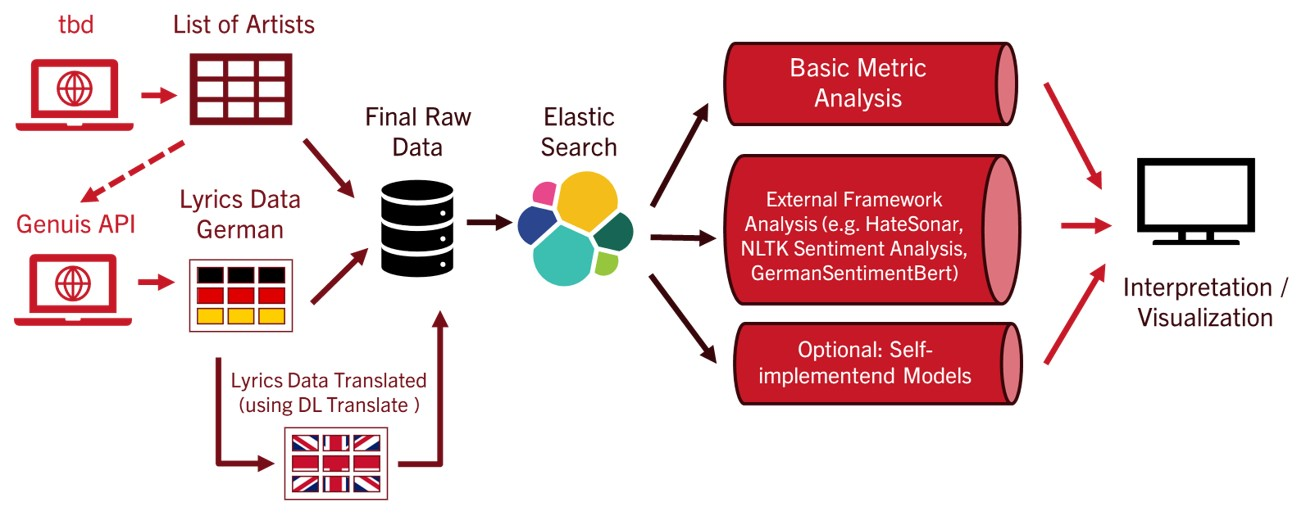
\includegraphics[width=\textwidth]{figures/pipeline.jpg}
  \caption[]{Text Analytics Pipeline}
  \label{fig:pipeline}
  \end{figure}

As a basis for our investigations, a data set on certain artists of the German Rap will be used, which is not finally defined yet. This will be done in the nearest future using information from the web in manual and partially automated work. Corresponding information about artists can be extracted, for example, from \cite{last.fm,tonspion_2021}. The names of those artists are used in a further step to download the lyrics of all songs of those artists via the song lyrics platform Genius \cite{genius}. Genius is an online database for any kind of artistic texts and offers an API interface that provides license-free lyrics of many song lyrics. Since Genius does not fully provide all the data of every international artist, it might be necessary to accept limitations for some artists.

The song lyrics, enriched with information about the artists themselves, finally form the basis of our textual analyses: Since we would like to use pretrained models for the analysis of the lyrics in a further step and many of these models only support English-language texts, it might be necessary to translate the German song lyrics first. For this, we intend to use the Python framework DL Translate \cite{lu_2022}, since it is the only package that can freely translate unlimited texts. The translated lyrics, will be stored together with the original lyrics in ElasticSearch. It must be taken into account that by using such a translation tool, possible linguistic-relevant contexts will be incorrectly transferred into the English language. However, since there is considerable interpretative space in the context of song lyrics, this limitation should not be of too much importance. In fact, it is important to keep in mind for the entire project that the song lyrics studied allow for different interpretations, which can only be determined by machine analysis to a limited extent.

As indicated in the paragraph before, we would like to store the translated song lyrics together with the original data in ElasticSearch. The possibilities that ElasticSearch offers in the area of tokenization, classification of words including counting of word frequencies, etc. shall then be used as a basis for a first analysis of the song lyrics.

In addition to the described methods offered by ElasticSearch, we would like to use predefined machine learning models to enrich the data of the song lyrics. In this context, the frameworks used should be considered as a black box, and the corresponding methods remain untouched. We will consider the following frameworks:

The project Deep Learning Models for Multilingual Hate Speech Detection \cite{deepMLhatespeech} includes multiple models that can be trained or fine-tuned for recognizing hate speech in various languages, especially German. Performing hate detection using different machine learning algorithms in parallel would enable a more thorough analysis of the texts like: highlighting songs that get a high hate rate from most models, identifying common patterns between such songs and classifying them into subclasses according to the target of the hate speech (foreigners, women, disabled people etc.).

The German Sentiment classification with BERT \cite{guhr2020training} is a sentiment classification model trained on around 1.8 million German-language text samples coming from various sources (social media, movie, app and hotel reviews). It could be a starting point for identifying potential hateful song lyrics. Given the three sentiment classes used by this model (negative, neutral and positive), we could filter out texts classified as positive and also separate negative from neutral lyrics for the upcoming pipeline stages.

NLTK.Vader \cite{vader} is an NLP algorithm trained for performing sentiment analysis. It is best suited for short texts like posts on social media, containing some slang and abbreviations. Hence, our dataset on German song lyrics would make a good fit for this model (providing we first use a translation model like mBart \cite{mBart}).

HateSonar \cite{davidson2017automated} is a BERT based model built with Python for hate speech detection. It only works with English data, therefore the German song lyrics would first need to be translated. As with models trained on German texts, it would be beneficial to the analysis to extract information regarding hate speech from multiple models.

If there is time left, we would like to develop independent machine learning models on our own using the methods discussed in the lecture. However, this requires classification of the existing lyrics data, which would likely need to be done manually. Furthermore, the amount of data available could prove challenging with this approach. If it is not feasible to identify a very large number of song lyrics using the listed approach above, it could be difficult to develop meaningful machine learning models.

Finally, the results of the different analysis methods will be interpreted and visualized. Thereby, the findings of the analyses shall be explicitly highlighted using the lyrics data by visual markers. Additionally, results of the different metrics will be displayed. 

\bibliographystyle{plain}
% b) The File:
\bibliography{references}

\end{document}
